% This example An LaTeX document showing how to use the l3proj class to
% write your report. Use pdflatex and bibtex to process the file, creating 
% a PDF file as output (there is no need to use dvips when using pdflatex).

% Modified 

\documentclass{l3proj}

\begin{document}

\title{An Example Project}

\author{Lewis Carroll \\
        Betty Davis \\
        James Dean \\
        Marilyn Monroe \\
        John Wayne}

\date{9 January 2009}

\maketitle

\begin{abstract}

The abstract goes here

\end{abstract}

%% Comment out this line if you do not wish to give consent for your
%% work to be distributed in electronic format.
\educationalconsent

\newpage

%==============================================================================
\section{Introduction}

Software engineering 

This paper presents a case study of... 


%% Final paragraph.
The rest of the case study is structured as follows.  Section
\ref{sec:background} presents the background of the case study
discussed, describing the customer and project context, aims and
objectives and project state at the time of writing.  Sections
\ref{sec:alice} through Section \ref{sec:managing} discuss issues that
arose during the project...

%==============================================================================
\section{Case Study Background}

Include details of 

\begin{itemize}
\item The customer organisation and background.
\item The rationale and initial objectives for the project.
\item The final software was delivered for the customer.
\end{itemize}

%==============================================================================
\section{Alice}
\label{sec:alice}

ALICE \cite{alice} was beginning to get very tired of sitting by her sister
on the bank and of having nothing to do: once or twice she had peeped into
the book her sister was reading, but it had no pictures or conversations in
it, ``and what is the use of a book,'' thought Alice, ``without pictures or
conversations?'

So she was considering, in her own mind (as well as she could, for the hot
day made her feel very sleepy and stupid), whether the pleasure of making a
daisy-chain would be worth the trouble of getting up and picking the
daisies, when suddenly a White Rabbit with pink eyes ran close by her.

There was nothing so very remarkable in that; nor did Alice think it so
very much out of the way to hear the Rabbit say to itself ``Oh dear! Oh
dear! I shall be too late!'' (when she thought it over afterwards it
occurred to her that she ought to have wondered at this, but at the time it
all seemed quite natural); but, when the Rabbit actually took a watch out
of its waistcoat-pocket, and looked at it, and then hurried on, Alice
started to her feet, for it flashed across her mind that she had never
before seen a rabbit with either a waistcoat-pocket, or a watch to take out
of it, and burning with curiosity, she ran across the field after it, and
was just in time to see it pop down a large rabbit-hole under the hedge.

In another moment down went Alice after it, never once considering how in
the world she was to get out again.

The rabbit-hole went straight on like a tunnel for some way, and then
dipped suddenly down, so suddenly that Alice had not a moment to think
about stopping herself before she found herself falling down what seemed to
be a very deep well.

Either the well was very deep, or she fell very slowly, for she had plenty
of time as she went down to look about her, and to wonder what was going to
happen next. First, she tried to look down and make out what she was coming
to, but it was too dark to see anything: then she looked at the sides of
the well, and noticed that they were filled with cupboards and
book-shelves: here and there she saw maps and pictures hung upon pegs. She
took down ajar from one of the shelves as she passed: it was labeled
``ORANGE MARMALADE'' but to her great disappointment it was empty: she did
not like to drop the jar, for fear of killing somebody underneath, so
managed to put it into one of the cupboards as she fell past it.

``Well!'' thought Alice to herself ``After such a fall as this, I shall think
nothing of tumbling down-stairs! How brave they'll all think me at home!
Why, I wouldn't say anything about it, even if I fell off the top of the
house!'' (which was very likely true.)

Down, down, down. Would the fall never come to an end? ``I wonder how many
miles I've fallen by this time?'' she said aloud. ``I must be getting
somewhere near the centre of the earth. Let me see: that would be four
thousand miles down, I think-'' (for, you see, Alice had learnt several
things of this sort in her lessons in the school-room, and though this was
not a very good opportunity for showing off her knowledge, as there was no
one to listen to her, still it was good practice to say it over) `` yes
that's about the right distance -- but then I wonder what Latitude or
Longitude I've got to?'' (Alice had not the slightest idea what Latitude
was, or Longitude either, but she thought they were nice grand words to
say.)

Presently she began again. ``I wonder if I shall fall fight through the
earth! How funny it'll seem to come out among the people that walk with
their heads downwards! The antipathies, I think-'' (she was rather glad
there was no one listening, this time, as it didn't sound at all the right
word) ``but I shall have to ask them what the name of the country is, you
know. Please, Ma'am, is this New Zealand? Or Australia?'' (and she tried to
curtsey as she spoke- fancy, curtseying as you're falling through the air!
Do you think you could manage it?) ``And what an ignorant little girl she'll
think me for asking! No, it'll never do to ask: perhaps I shall see it
written up somewhere.''

Down, down, down. There was nothing else to do, so Alice soon began talking
again. ``Dinah'll miss me very much to-night, I should think!'' (Dinah was
the cat.) ``I hope they'll remember her saucer of milk at tea-time. Dinah,
my dear! I wish you were down here with me! There are no mice in the air,
I'm afraid, but you might catch a bat, and that's very like a mouse, you
know. But do cats eat bats, I wonder?'' And here Alice began to get rather
sleepy, and went on saying to herself, in a dreamy son of way, ``Do cats eat
bats? Do cats eat bats?'' and sometimes ``Do bats eat cats?'' for, you see, as
she couldn't answer either question, it didn't much matter which way she
put it. She felt that she was dozing off, and had just begun to dream that
she was walking hand in hand with Dinah, and was saying to her, very
earnestly, ``Now, Dinah, tell me the truth: did you ever eat a bat?'' when
suddenly, thump! thump! down she came upon a heap of sticks and dry leaves,
and the fall was over.

Alice was not a bit hurt, and she jumped up on to her feet in a moment: she
looked up, but it was all dark overhead: before her was another long
passage, and the White Rabbit was still in sight, hurrying down it. There
was not a moment to be lost: away went Alice like the wind, and was just in
time to hear it say, as it turned a comer, ``Oh my ears and whiskers, how
late it's getting!'' She was close behind it when she turned the comer, but
the Rabbit was no longer to be seen: she found herself in a long, low hall,
which was lit up by a row of lamps hanging from the roof.

There were doors all round the hall, but they were all locked; and when
Alice had been all the way down one side and up the other, trying every
door, she walked sadly down the middle, wondering how she was ever to get
out again.

Suddenly she came upon a little three-legged table, all made of solid
glass: there was nothing on it but a tiny golden key, and Alice's first
idea was that this might belong to one of the doors of the hall; but, alas!
either the locks were too large, or the key was too small, but at any rate
it would not open any of them. However, on the second time round, she came
upon a low curtain she had not noticed before, and behind it was a little
door about fifteen inches high: she tried the little golden key in the
lock, and to her great delight it fitted!

\begin{figure}
\begin{center}
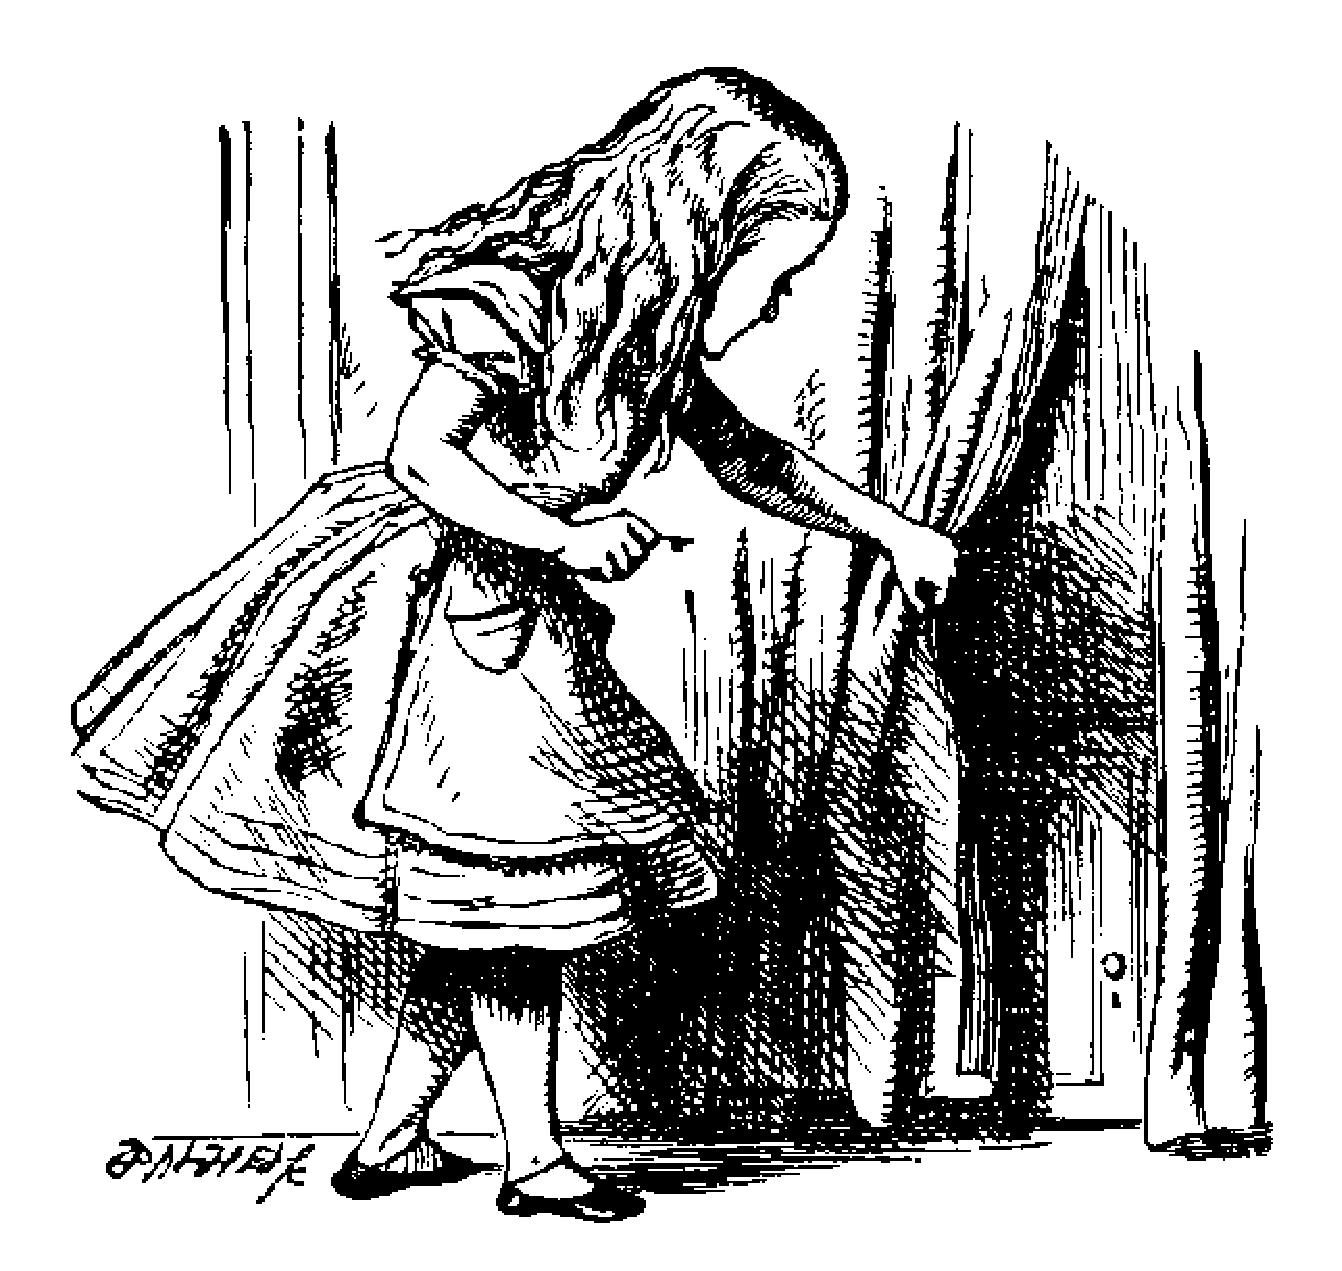
\includegraphics[width=7cm]{figures/alice}
\end{center}
\caption{Behind it was a little door}
\label{fig:alice}
\end{figure}

Alice opened the door (see Figure \ref{fig:alice}) and found that it
led into a small passage, not much larger than a rat-hole: she knelt
down and looked along the passage into the loveliest garden you ever
saw. How she longed to get out of that dark hall, and wander about
among those beds of bright flowers and those cool fountains, but she
could not even get her head through the doorway; ``and even if my head
would go through,'' thought poor Alice, ``it would be of very little
use without my shoulders. Oh, how I wish I could shut up like a
telescope! I think I could, if I only knew how to begin.'' For, you
see, so many out-of-the- way things had happened lately, that Alice
had begun to think that very few things indeed were really impossible.

Iteration One and Two

We spent Iteration One with getting set up and getting to know each other better to identify each others’ strengths  in order to assign technical tasks efficiently in the future.
We set up our GitLab account, installed the virtual machine on the lab machines and familiarised ourselves with Linux.
We also created a Slack account in order to communicate efficiently in the future on multiple channels and participated on a 48-hour Hackathon, partly as a team building exercise.  

Iteration Two started with the team being assigned to our customer, Cooper Software. The goal for the end of this iteration was to have a detailed backlog, consisting of the detailed description of the project, and a clear well-organised set of tasks in GitLab to start delivering features.
The first step was to gather requirements, for which we needed frequent contact with the representative of Cooper Software. Since our customer was based 70 miles away, we decided that the best way to keep in touch would be on Slack with occasional video conferences.
As expected in the initial requirements gathering phase, features and requirements were added, removed and changed on an ongoing basis. Requirements gathering was an iterative process, in which the team gradually increased clarity about the required features and its priorities.
In order to foster the creation of a common understanding of the requirements, we decided to create various forms of documentation in order to ensure that we are on the same page with the customer. We created:
User Personas who represent the primary types of users who would interact with the app we would build.
An initial architecture diagram which would explain the general information flow of the application.
Wireframes, using a method our coach suggested: 
Each member of the team drafted five possible wireframes for the main page of the app, then explained his ideas to the rest of the team. After that, each member of the team drafted two suggested wireframes and explained his decisions to the rest of the team.
Finally everybody was required to draft one wireframe, and to everyone’s relief the proposed wireframes converged significantly.
User stories for the main features of the app. As per the request of our customer, we aimed to have user stories written from a non-technical end user perspective. Each user story was designed to be as atomic as possible, with the terse structure of “As a < type of user>, I want to <action describing feature>, So that <action describing benefit of feature>”
A very helpful technique we employed here was the Value Proposition Canvas, which helped us empathise with the customer, identify the core business value the application was creating, and the issues it was meant to resolve. This knowledge helped us tailor our solutions to the customer’s needs.
As suggested in the Principles behind the Agile Manifesto, we welcomed changing requirements.
The final documentation is the result of many iterations of the following process:

Creating documentation artifacts
Discussing the documentation artifacts with the customer
Taking notes of new or changed requirements

Following that, we used the MoSCoW method to identify the most important features to implement in the coming iteration as “Must-Haves”. These were: 
basic web app
create predefined template
prototype for file conversion from PDF to JSON via predefined template

We uploaded all the gathered requirements and produced documentation to the Wiki page of GitLab.  Initially, we uploaded the list of user stories to the wiki as well, and we added technical tasks to be done to deliver features to the board with labeled due dates.

We started to diversify our communication to multiple channels on Slack to reflect the growing complexity of the project: we prepared for the coming meeting with the customer on the channel #presentation, while we created a very handy channel #guides, where we copied useful commands and reference guides, e.g. how to log in to the VM, how to install a virtual environment and dependencies, recurrent git commands, etc.

Since occasions to meet the customer in person were scarce, we tried to maximise the benefits of the customer meeting by having a well-structured presentation of our accomplishments thus far and our planned deliverables for the coming iteration. We planned the meeting so that each team member would get to talk about their share of tasks in the first half of the meeting and we would have time for an open discussion with the customer in the second half. However the customer preferred to have a dialogue-like meeting throughout, which made us to improvise on the spot. The meeting overall went very well, but having learnt from the experience of the first customer meeting, we decided that in following meetings we would share the responsibilities differently: one team member would present the slides, two team members would respond to the customer’s questions and ask for clarifications/more details in case of new requirements, and two team member would act as observers/note takers.

After the customer meeting, we also had our first retrospective. Retrospectives are crucial for a modern software development process; they force the developers to look at the bigger picture, ironing out the methods and practices employed by the team so that productivity and efficiency is maximized. They give team members a chance to vocalise any grievances they might have had during the development process in the appropriate time and environment. Airing grievances at an inappropriate time can make a developer feel insecure, whereas proper retrospective meetings allow for a healthier environment for criticism and self improvement.

Frameworks are a great help with structuring retrospectives. A retrospective framework describes a technique by which all team members offer their criticism in organised manner that allows the complaints to be grouped according to categories by the end of the meeting. For this specific retrospective, we employed the “Liked-Learned-Lacked-Longed For” framework. One of the ways that a retrospective allows for a healthy environment is by including positive remarks that balance out the negativity of the complaints. Remarks by the team are written under the four columns, which scale according to importance from left to right. Ideally, the team will learn some useful lessons from the retrospective and successfully hone their teamwork skills. In hindsight, we conclude that our first retrospective had vague suggestions and criticisms, and we did not identify solutions to the issues raised.




Iteration Four

This iteration spans across two months so as a team, we decided to split it between two shorter sprints, one which goes across the December break and one that covers the rest. Since it was the longest iteration and we had met all our objectives in the previous iteration, we set goals that, compared to the other iterations, were more ambitious.

Everyone went back home for holidays and/or took a break which made communications a bit harder but prior to going back, the team had assigned clear tasks to each other which are also tracked in the issue board. We also started using planning poker, and added the estimated delivery efforts as numbers next to each issue. This organisation helped us stay motivated during this long period of time being physically separated. However, during the middle of the break, there was a disruption to the university network which rendered us unable to access the repository as well as the issue tracking system which hindered the progress of the team as not only we were unable to access the latest file or update the repository, we were also not able to track issues which is necessary for task delegation until the break was over. We decided to move to a temporary repository on the public Gitlab and later migrating back to the university Gitlab. Since the team was not too experienced in migrating repositories, despite the files being successfully migrated, the process was not smooth. The commits pushed during the server downtime are only accessible in the temporary GitLab repository, the are not visible in the main GitLab repository. 

One of the main tasks was to develop a template creator, an interactive drawing app within the web app that would allow users to define areas within the PDFs that would be processed by the main application. This would later be accompanied by a template editor where users can load up previously defined templates to edit the properties. The template creator was done during the break with improvements to be made in the future and the template editor came a bit later and it was found out many parts of the code were repetitive between the two so the team decided to do code reviews on it so that refactoring can be done in order to follow the principle of Don’t Repeat Yourself (DRY).

The other main tasks for the web app in the iteration were to develop the back end by implementing numerous back-end functions, database and also trying to move some external functions into the web application to ensure the application would perform consistently across multiple platforms (this was found to be a problem before migrating external functions as the OCR would produce different output on Windows and Linux). Furthermore, we set up a user system as in the design of the project, the application was designed to have two different users, regular user and admin (superuser). All of the above tasks were achieved within the iteration.

Additional goals include development for the main page (the page containing the result of processing PDF) and general error checking. A few missed objectives include user friendly representation of JSON data on the main page, error checking when PDF is converted into JSON and a few bugs on the template creator. 

As the team got more used to the Gitlab system, we developed and improved the continuous integration pipeline and as requested by the customer, the pipeline was to be designed to also produce an artifact that would allow the customer to be able to deploy the latest build of the software. In order to improve user friendliness, a user guide was required that would make it easier for the customer to deploy. The pipeline would try to build the software from scratch every time a commit was made, this is necessary to make sure that every time a change has been made, the software would not break when being installed on a new system.

The team also decided to step up on the quality assurance department and one of the goals in the iteration was to achieve high test coverage across the files by filling it up with meaningful tests. Having a high-test coverage would reduce defects as almost every single part of the code would be tested every time the test suite was activated, which occurs with every commits to the repository as it is attached to the continuous integration pipeline. This means that every time an update was made to the codebase and parts were changed, we can ensure that it does not break other parts of the code and this reduces the risk overall.

The iteration ended with another successful demonstration to the customer, followed by a retrospective. During the retrospective, the team used starfish technique following the suggestion of the team coach. This retrospective contains five different sections, namely: Start, Stop, Continue, More of and Less of. The team agreed to:
Start doing dissertation studies and communicate via issues
Stop pushing too late before the meeting and stop being late to the meetings
Less of being distracted in meetings
More of testings, code reviews, comments, motivation, making sure VM works
Keep doing great demos, good communication and task delegation
One realization we had after the retrospective was that we were not keeping clear track of how well we are implementing the solutions the team agreed to have after the previous retrospective. The solution to this is that the team decided to have a different type of issue labelled as “Retrospective Solutions” on the issue board, moving them between stages similarly to any other issues on subsequent meetings, as we assessed ourselves how good we are at sticking to the identified solutions. We found that this method of suggesting concrete solutions and adhering to them greatly improved our efficiency, communication and teamwork skills. For example, to avoid becoming distracted, a constructive solution was to try to implement the pomodoro method. Overall, the team managed to accomplish most of the tasks set for the iteration and was able to follow up on most of the retrospective solutions despite a few hiccups.
%==============================================================================

\section{Choice of Colours}
\label{design}

The following diagrams (especially figure \ref{fig:alice}) illustrate the
process...

%==============================================================================
\section{Managing Dress Sense}
\label{managing}

In this chapter, we describe how the implemented the system.

%------------------------------------------------------------------------------
\section{Kangaroo Practices}



% - - - - - - - - - - - - - - - - - - - - - - - - - - - - - - - - - - - - - - -
\section{Knots and Bundles}
\label{sec:managing}


%------------------------------------------------------------------------------
\section{Conclusions}

In hindsight, the conclusions we can draw can be enumerated as follows:
Initial requirements gathering and planning phase
Requirements are very fuzzy in the beginning, as the project takes shape. Project documentation, such as user personas, wireframes, site URLs, UML diagrams take time, but help immensely to create clarity between the development team and the customer.
Once the initial requirements are agreed, it is a good idea to produce a quick prototype. This gives the customer the opportunity to further clarify requirements, and the team to quickly change and adopt to these. Following a successful prototype and agreed requirements, it is useful to identify the scope of the project and decide on web frameworks to use. Django was an excellent choice for the backend, however we would have benefited from a front-end framework such as React or Angular for multiple users: automated testing would have been very easy to implement and we could have enjoyed better library and community support.
Project Management and Development

As it was expected, Team Dynamics evolved throughout the course of the project: as we got to know each better, and got used to working together, we could better estimate the delivery costs of certain features and our understanding of the frameworks and tools we used increased too. We found retrospectives the best tools to improve our team work, especially when we decided to suggest concrete solutions to the identified issues and adhered to them improved the teams commitment and efficiency in the project. 

Quality Assurance
Although the backend is thoroughly tested with over 90\% coverage, our front-end lacks tests. This is partly due to not using any front-end frameworks, partly to occasionally prioritising delivering features over thorough tests.
We started user-testing late, which revealed several bugs at the end of the project. Due to the complexity and unusual nature of the app (it is meant to be used in a company not be usual end users), user testing was difficult to organise and get useful results. Each user test would first need a thorough debrief and setup, which is fairly time-consuming and resource-intensive. An alternative option could have been to gather 10-15 users into one physical place, debrief them and make them test the app at once in order to save time and introduce competition among them to think of unusual edge cases to be tested.

Since the start of our degrees, the Team Project was possibly our biggest step up in our journey to become professional software developers. This was the first time we worked in a reasonably large group for an extended amount of time creating software for a real world customer. Over the course of the project, we got to learn new technologies, such as CI/CD, various python and javascript libraries and we had the chance to apply the principles and practices learnt during the Professional Software Development course. We feel that having worked in a small agile team for two semesters gave us the communication, teamwork skills and industry best practices knowledge to perform well in our summer internships / year placements.


%==============================================================================
\bibliographystyle{plain}
\bibliography{dissertation}
\end{document}
